\section{Durchführung}
\label{sec:Durchführung}
\subsection{Magnetfeld von Spulen}
Zuerst wird eine Spule an das Netzgerät angeschlossen und eine bestimmte
Spannung und einen bestimmten Strom eingestellt. Dabei ist es wichtig den maximalen
zulässigen Strom der Spule nicht zu überschreiten.
Nun wird eine logitudinale Sonde an der Halterung befestigt. Die Spule wird auf das Lineal gestellt, so dass
die Sonde am Anfang der Spule misst (wie in Abbildung \ref{fig:spule_lang} zu sehen). Der Ort wird als $x=0$ gewählt.\\
Jetzt wird die magnetische Feldstärke abgelesen und notiert. Im Anschluss wird die Spule um $\Delta x = \SI{0.5}{\cm}$ verschoben und
nochmal die Feldstärke gemessen. Insgesamt sollten mindestens 10 Werte innerhalb und ein paar Werte außerhalb der Spule gemessen werden.
Um bei der Auswertung einen Plot zu erhalten der die ganze Spule abbildet, sollte die lange Spule gedreht und das Feld gemessen werden.
Bei der Drehung der Spule wird das Koordinatensystem um die länge der Spule verschoben und die Ausrichtung der x-Achse verdreht.
\begin{figure}
    \centering
    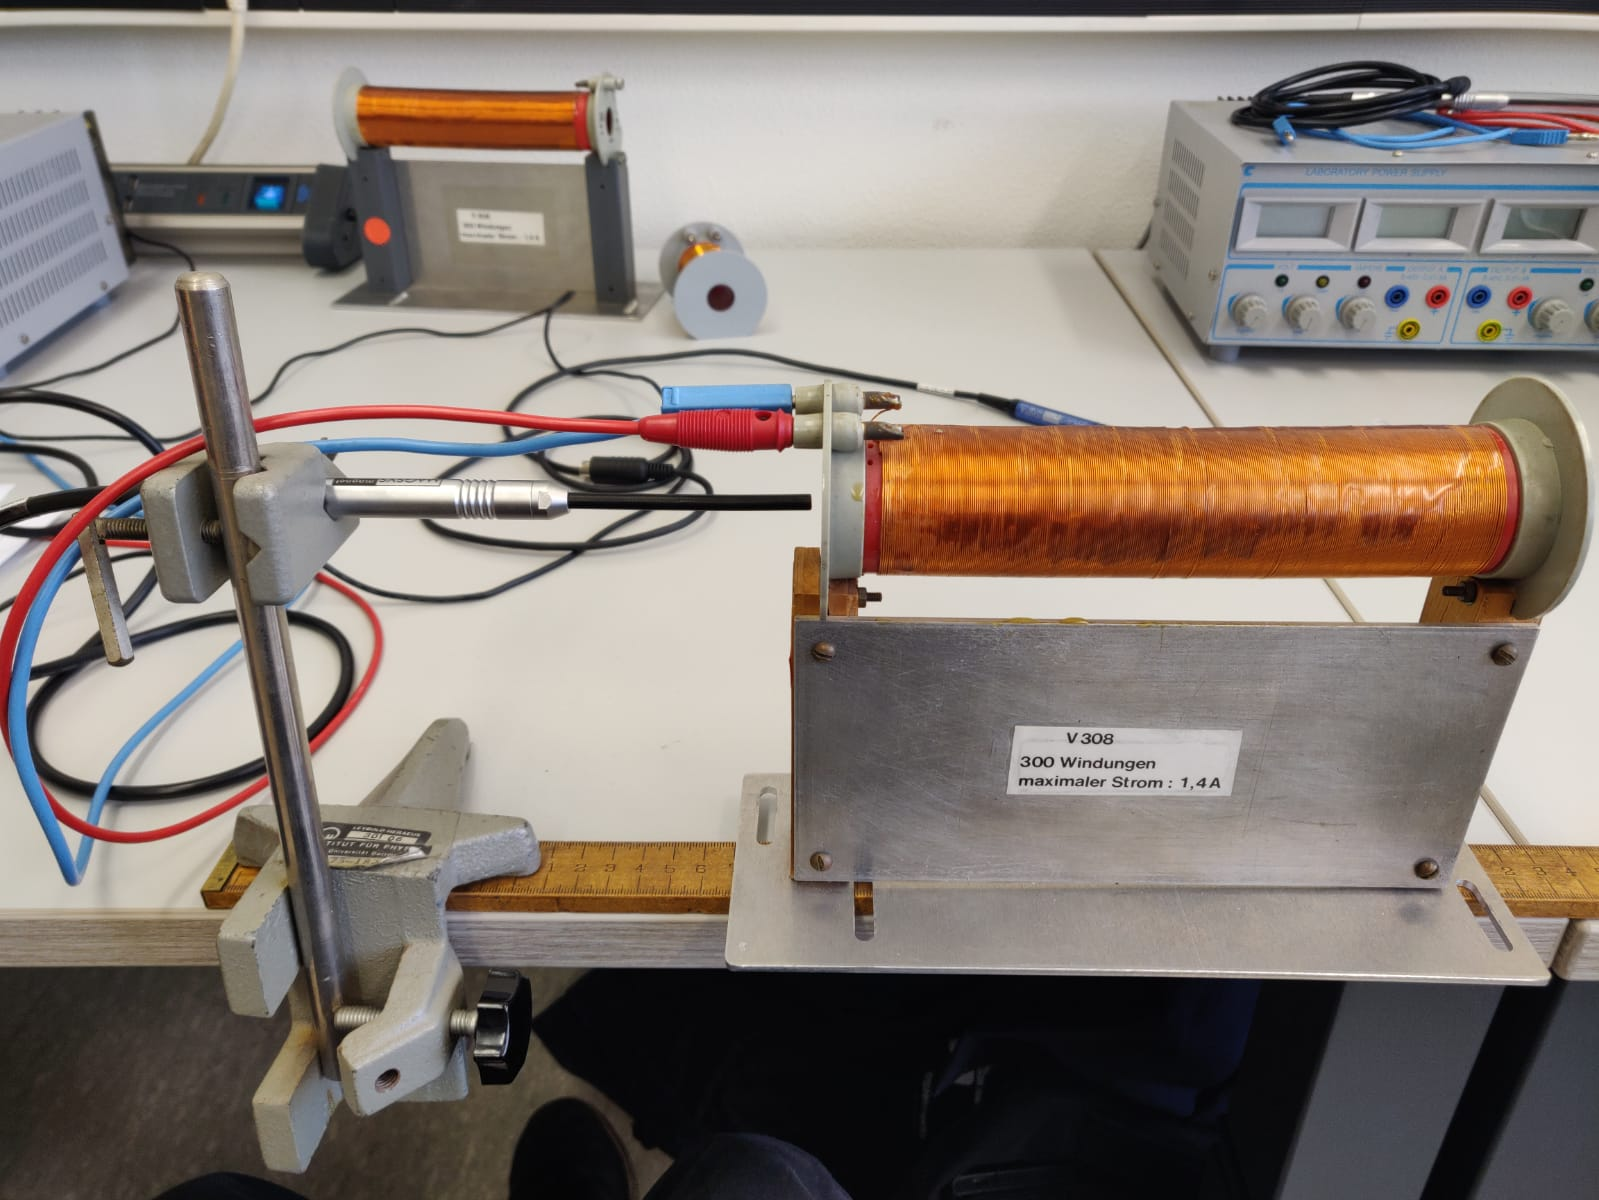
\includegraphics[height=6cm]{content/spule_lang.jpg}
    \caption{Versuchsaufbau um das Magnetfeld einer Spule mit einer Hall-Sonde zu messen.}
    \label{fig:spule_lang}
\end{figure}
\FloatBarrier
\subsection{Magnetfeld eines Spulenpaares}
Das Spulenpaar wird an das Netzgerät angeschlossen und ein Strom $I$ und eine Spannung $U$ wird eingestellt.
Um die Spulen nicht zu überlasten sollte der Strom unter $\SI{5}{\ampere}$ gehalten werden.
Von oben wird eine transversale Hall-Sonde zwischen die Spulen montiert (siehe Abbildung \ref{fig:spulenpaar}).
\begin{figure}
    \centering
    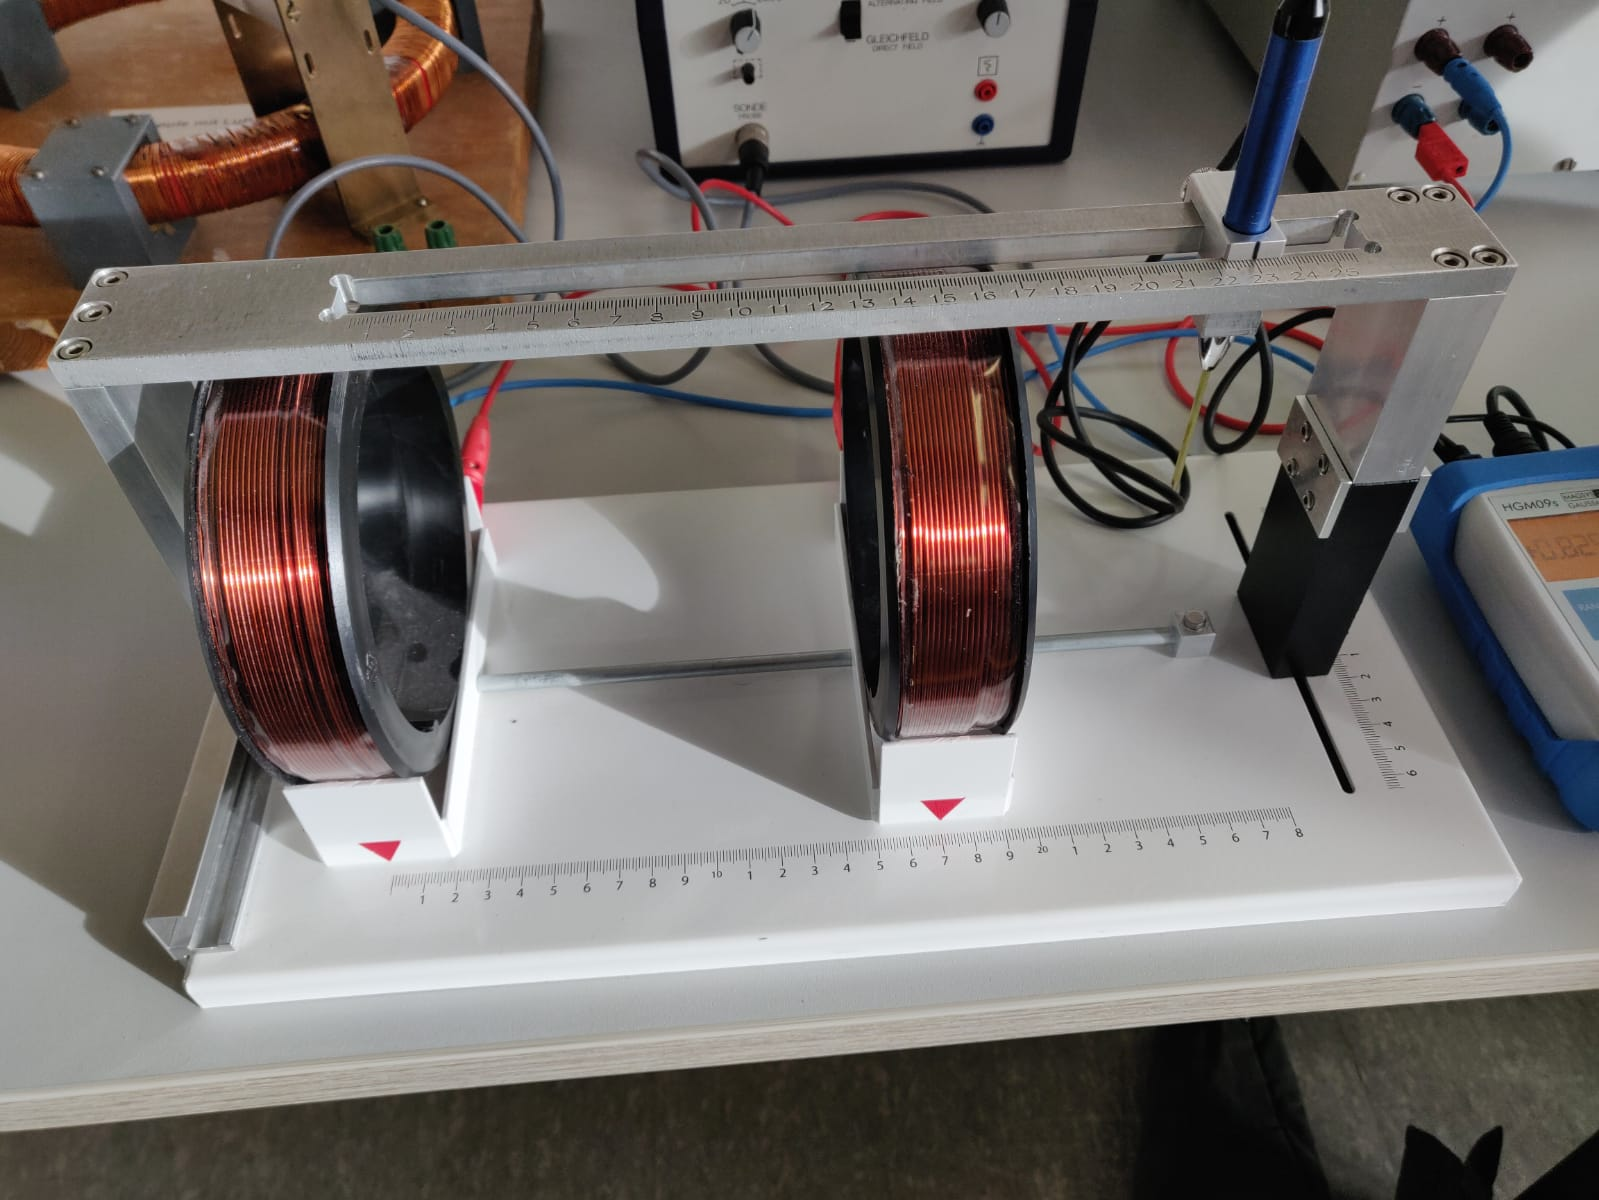
\includegraphics[height=6cm]{content/spulenpaar.jpg}
    \caption{Spulenpaar mit Abstand $d$ und Radius $R$, mit transversaler Hall-Sonde.}
    \label{fig:spulenpaar}
\end{figure}
\FloatBarrier
Wichtig dabei ist, dass die Sensoren der Hall-Sonde genau Richtung Spulen zeigen.
Jetzt wird ein wählbarer Spulenabstand eingestellt und das Magnetfeld innerhalb der Spulen und außerhalb der Spulen gemessen.
Dieser Vorgang wird mit zwei weiteren Abständen durchgeführt.

\subsection{Hysteresekurve}
Zuerst wird die Ringspule mit dem Netzgerät verbunden und ein Strom $I$ eingestellt. Hier ist keine externe Hall-Sone notwendig,
da bereits eine festmontierte transversale Hall-Sonde in der Spule verbaut ist. (Abbildung \ref{fig:hysterese}) 
Um die Neukurve darstellen zu können, wird zuerst die Magnetisierung des Eisenkerns der Spule durch ein Gegenfeld
kompensiert und umgepolt, bis kein magnetisches Feld mehr zu messen ist. Dann werden folgende Messungen getätigt
\begin{figure}
    \centering
    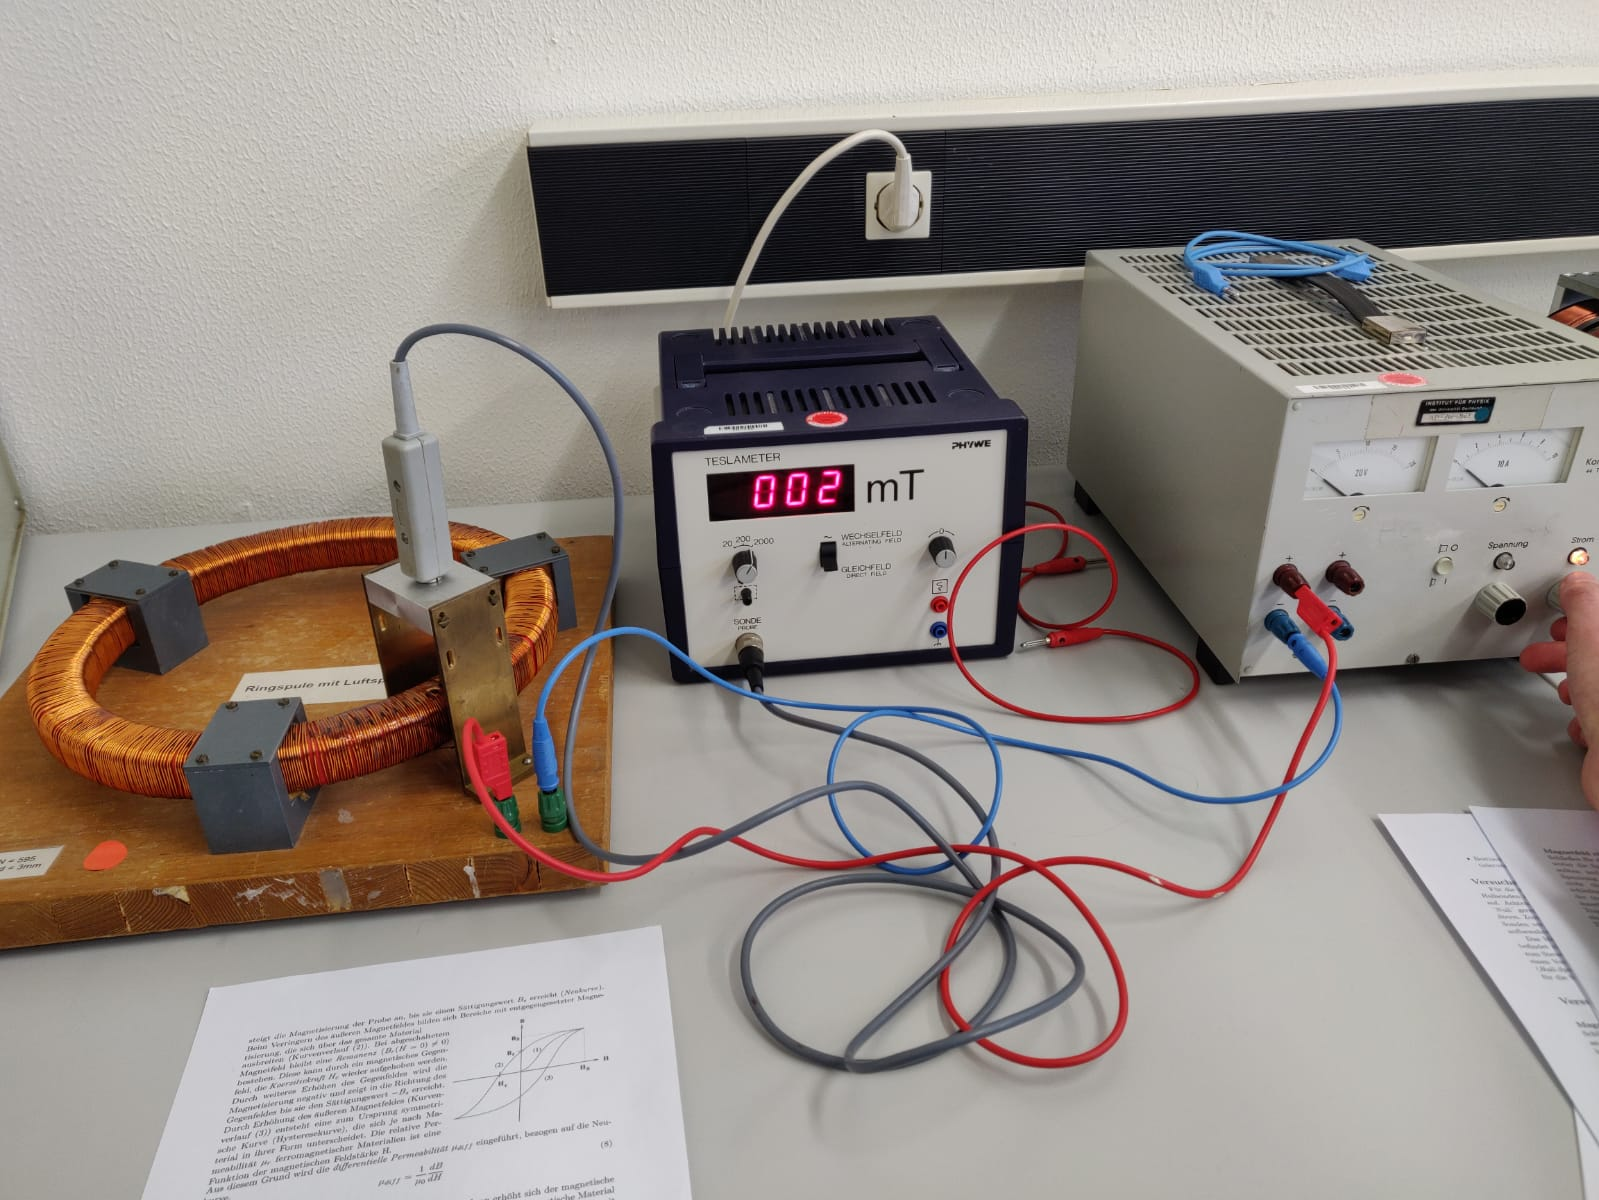
\includegraphics[height=6cm]{content/ring.jpg}
    \caption{Versuchsaufbau für die Messung der Magnetfeldstärke für die Ringspule mit Eisenkern.}
    \label{fig:hysterese}
\end{figure}
\FloatBarrier
\begin{enumerate}
    \item Der Strom wird in $\SI{1}{\ampere}$-Schritten erhöht und das Magnetfeld gemessen und notiert, bis $\SI{10}{\ampere}$ erreicht sind.
    \item Strom in $\SI{1}{\ampere}$-Schritten verringern bis kein Strom mehr fließt. Dann Richtung
    des Stromfluss vertauschen um ein Gegenfeld zu erzeugen. Auch hier wird wieder von 1 bis 10 Volt das Magnetfeld gemessen und notiert.
    \item Nun den Strom in $\SI{1}{\ampere}$ Schritten reduzieren und das Magnetfeld messen bis wieder 0 Volt erreicht sind. Dann das Feld erneut umpolen
    und die magnetische Feldstärke in $\SI{1}{\ampere}$ Schritten messen und notieren.
\end{enumerate}